\section{Weiterführende Themen}
\subsection{Sensoren}
Bewegungs-, Umgebuns- und Lagesensoren.
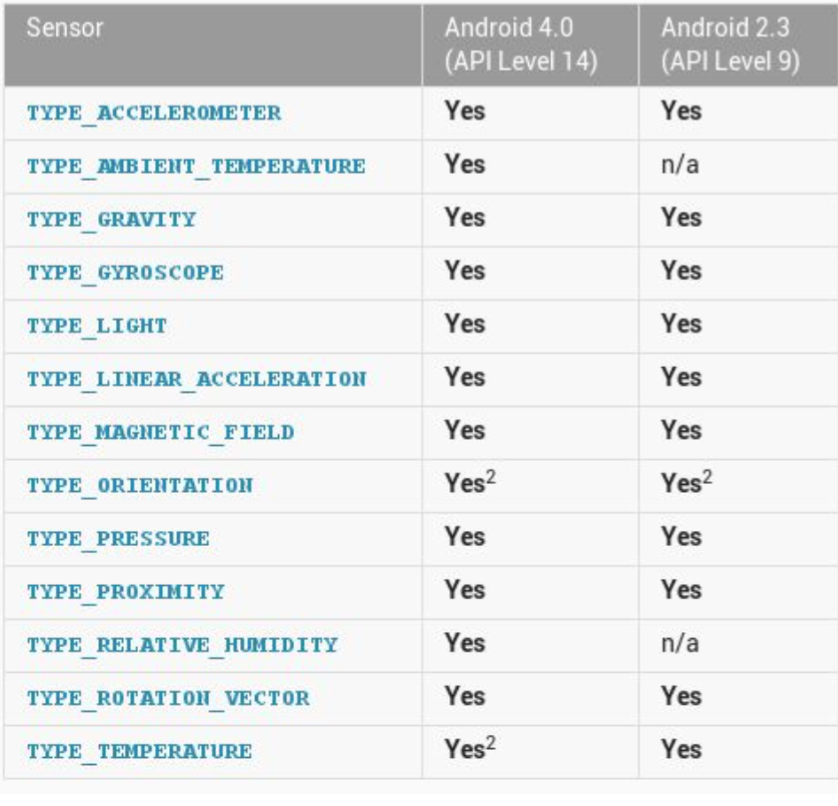
\includegraphics[scale=0.35]{sensors.png} \\
Für die Arbeit mit einem Sensor brauchen wir:
\begin{itemize}
\item \code{SensorManager} als Einstiegspunkt für die Sensoren
\item \code{Sensor} als Repräsentant für einen konkreten Sensor
\item \code{SensorEventListener} um Updates von Sensoren zu registrieren
\item \code{SensorEvent} um die Sensordaten auszulesen
\end{itemize}
Ein Sensor liefert uns nur Rohdaten! Je nach Sensor unterschiedlich zu interpretieren. Sensor Bsp.:
\begin{lstlisting}
public class MainActivity extends AppCompatActivity implements SensorEventListener {
   private TextView textView;
   private SensorManager sensorManager;
   private Sensor lightSensor;
   @Override
   protected void onCreate(Bundle savedInstanceState) {
       ...
       textView = (TextView) findViewById(R.id.textView);
       sensorManager = (SensorManager) getSystemService(Context.SENSOR_SERVICE);
       lightSensor = sensorManager.getSensorList(Sensor.TYPE_LIGHT).get(0);
   }
   @Override
   protected void onResume() {
       super.onResume();
       sensorManager.registerListener(this, lightSensor, SensorManager.SENSOR_DELAY_NORMAL);
   }
   @Override
   protected void onPause() {
       super.onPause();
       sensorManager.unregisterListener(this);
   }
   @Override
   public void onSensorChanged(SensorEvent event) {
       textView.setText(String.format("Helligkeit: %.0f", event.values[0]));
   }
}
\end{lstlisting}
\subsection{View Injection}
Flexible Lösung wäre Service ausserhalb der Activity zu erstellen und dieser übergeben. Noch besser: Interface von LibraryService extrahieren und im Test durch einen Fake-Server ersetzen. Die Klasse erstellt seine Dependencies also nicht selbst, stattdessen werden diese injiziert (injected). \\
Einfache Lösung: Konstruktor mit Parametern und final-Attributen. Stellt sicher das Klasse vollständig initialisiert wurde. \\
Weniger Schön: Setter Methoden. Benutzer muss aufpassen das alle aufruft. \\
Dagger Tool verwenden: \textbf{Modul} instanziert unsere Klasse(z.B. LibraryService) die wir injecten wollen. \textbf{Komponente} fasst Module zusammen und ist zuständig für die Injection. Eine Klasse lässt sich über die Komponenten ihre Abhängigkeiten injecten.
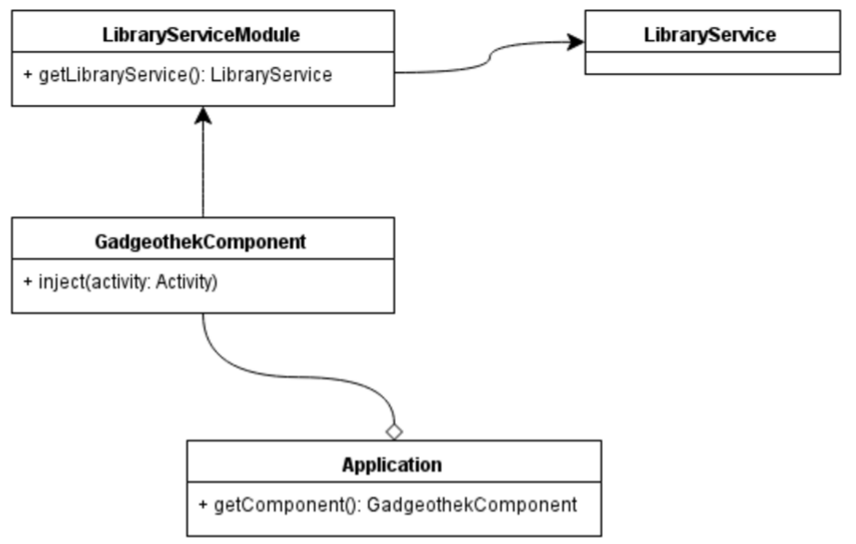
\includegraphics[scale=0.35]{Injection1.png} \\
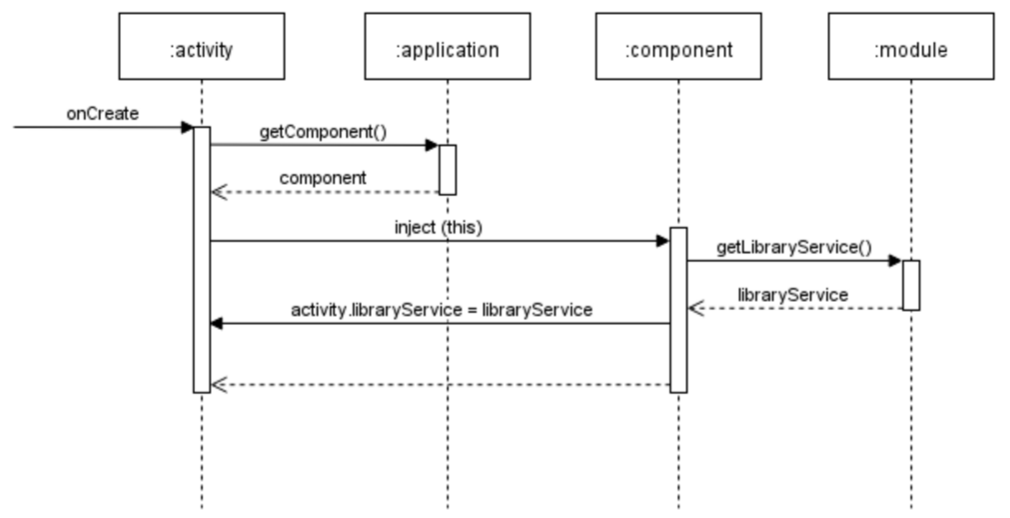
\includegraphics[scale=0.35]{Injection2.png}
\begin{lstlisting}
@Module
public class LibraryServiceModule {
   @Provides
   @Singleton
   public LibraryService getLibraryService() {
       return new LibraryService();
   }
}


@Singleton
@Component(modules = {LibraryServiceModule.class})
public interface GadgeothekComponent {
   void inject(GadgeothekActivity activity);
}
\end{lstlisting}
\begin{lstlisting}
public class Application extends android.app.Application {
   GadgeothekComponent component;

   public void onCreate() {
       component = DaggerGadgeothekComponent.builder().build();
   }

   public GadgeothekComponent getComponent() {  return component;  }
}


public class GadgeothekActivity extends AppCompatActivity {

   @Inject
   LibraryService libraryService;

   @Override
   protected void onCreate(Bundle savedInstanceState) {
   ...
   ((Application) getApplication()).getComponent().inject(this);
\end{lstlisting}
Lohnt sich Dependency Injection? \\
Vorteile:
\begin{itemize}
\item keine statischen Methoden mehr
\item zentrale Konfiguration in Modul und Komponente
\item Einfache Testbarkeit: Modul oder Applikation austauschen
\end{itemize}
Nachteile:
\begin{itemize}
\item Nicht unbedingt weniger Schreibaufwand bei kleinen Projekten
\item Braucht Tests: bei einer Fehlkonfiguration drohen NullPointerException
\item Spaghetticode?
\end{itemize}
\subsection{Data Binding}
\begin{itemize}
\item erspart Tipparbeit
\item in XML direkt auf Objekte zugreifen (Bsp. \code{onClick})
\item Optimal: GUI aktualisiert sich selbst, sobald Objekt sich ändert
\begin{itemize}
\item XML-Layout als Observer
\item Einfache Logik (x ? y : z) direkt im XML
\end{itemize}
\item noch Beta
\end{itemize}
\begin{lstlisting}
public class User {
   public String firstName;
   public String lastName;

   public User(String firstName, String lastName) {
       this.firstName = firstName;
       this.lastName = lastName;
   }
}
\end{lstlisting}
\begin{lstlisting}
<layout xmlns:android="http://schemas.android.com/apk/res/android">
   <data >
       <variable name="user" type="ch.hsr.mge.databindingdemo.User"/>
   </data>
   <RelativeLayout
       ... >

       <TextView android:text="@{user.firstName}" ... />

       <TextView android:text="@{user.lastName}"  ... />
   </RelativeLayout>
</layout>
\end{lstlisting}
Expression Language unterstützt fast alle Java Expressions (Keine Statements Deklarationen, Loops, kein new, this und super)
\begin{lstlisting}
android:text="@{String.valueOf(index + 1)}"
android:visibility="@{age < 13 ? View.GONE : View.VISIBLE}"
android:transitionName='@{"image_" + id}'
\end{lstlisting}
\begin{lstlisting}
public class MainActivity extends AppCompatActivity {

   @Override
   protected void onCreate(Bundle savedInstanceState) {
       super.onCreate(savedInstanceState);

       ActivityMainBinding binding = 
           DataBindingUtil.setContentView(this, R.layout.activity_main);

       User user = new User("Mirko", "Stocker");
       binding.setUser(user);
   }
}
\end{lstlisting}
Neben Properties können auch Events gebunden werden
\begin{lstlisting}
<Button
   android:text="Save"
   android:onClick="@{controller.onButtonSaveClicked}"/>
   <EditText
   android:text="@{user.lastName}"
   android:addTextChangedListener="@{user.lastNameWatcher}" />
\end{lstlisting}
Was wenn gebundene Objekt sich ändert?
\begin{lstlisting}
public class User {
   public String lastName;
   public boolean isDirty;
  
   public TextWatcher lastNameWatcher = new TextWatcher() {
       @Override
       public void beforeTextChanged(CharSequence s, int start, int count, int after) { }

       @Override
       public void onTextChanged(CharSequence s, int start, int before, int count) {
           lastName = s.toString();
       }

       @Override public void afterTextChanged(Editable s) { }
   };
}
\end{lstlisting}
Um Daten aus gebundenen Objekten in der View zu aktualisieren benötigen wir wieder das Observer-Pattern. \textbf{View} observiert das gebundene Objekt. \textbf{Objekt} ist observable. Um unser Objekt observable zu machen müssen wir \code{ObservableFields} verwenden.
\begin{lstlisting}
public class User {
   public ObservableField<String> firstName = new ObservableField<>();
   public ObservableField<String> lastName  = new ObservableField<>();

   public TextWatcher lastNameWatcher = new TextWatcher() {
   ...
          if (!Objects.equals(lastName.get(), s.toString())) {
              lastName.set(s.toString());
          }
   }
};
\end{lstlisting}